%──────────────────────────────────────────────────────────────
%  CV — Daniël van Ginneken (Nederlands)
%──────────────────────────────────────────────────────────────
\documentclass[a4paper,10pt]{article}

% ── Packages ─────────────────────────────────────────────────
\usepackage[T1]{fontenc}
\usepackage[utf8]{inputenc}
\usepackage[margin=0.55in, top=0.45in, bottom=0.45in]{geometry}
\usepackage{titlesec}
\usepackage{enumitem}
\usepackage{hyperref}
\usepackage{xcolor}
\usepackage{fontawesome5}
\usepackage{tabularx}
\usepackage{parskip}
\usepackage{microtype}
\usepackage{graphicx}
\usepackage{tikz}
\usepackage{lmodern}

% ── Colours ──────────────────────────────────────────────────
\definecolor{accent}{HTML}{1B2A4A}
\definecolor{lightgray}{HTML}{555555}
\definecolor{ruleclr}{HTML}{CCCCCC}
\definecolor{taggray}{HTML}{888888}

% ── Hyperlinks ───────────────────────────────────────────────
\hypersetup{
  colorlinks=true,
  urlcolor=accent,
  linkcolor=accent,
  pdfauthor={Daniël van Ginneken},
  pdftitle={CV — Daniël van Ginneken},
}

% ── Section formatting ───────────────────────────────────────
\titleformat{\section}
  {\normalsize\bfseries\color{accent}\sffamily}
  {}{0pt}{\MakeUppercase}[\vspace{2pt}\textcolor{ruleclr}{\rule{\linewidth}{0.5pt}}]
\titlespacing*{\section}{0pt}{10pt}{4pt}

% ── Custom commands ──────────────────────────────────────────
\newcommand{\cventry}[4]{%
  {\textbf{#1}}\hfill{\small\color{lightgray}#2}\\
  {\small\color{lightgray}\textit{#3}}\hfill{\small\color{lightgray}#4}\vspace{2pt}%
}
\newcommand{\cvsimple}[2]{%
  {\textbf{#1}}\hfill{\small\color{lightgray}#2}\vspace{1pt}%
}
\newcommand{\contactitem}[2]{\mbox{#1\,\small #2}}

\pagestyle{empty}
\setlist[itemize]{leftmargin=14pt, itemsep=1pt, parsep=0pt, topsep=2pt}

\begin{document}

% ═══════════════════════════════════════════════════════════
% HEADER
% ═══════════════════════════════════════════════════════════
\noindent
\begin{minipage}[c]{0.78\textwidth}
  {\LARGE\bfseries\sffamily\color{accent} Daniël van Ginneken}\\[5pt]
  {\small\color{lightgray}Backend-gerichte softwareontwikkelaar · Oudenbosch, Nederland}\\[5pt]
  \contactitem{\faEnvelope}{\href{mailto:dcjvanginneken@gmail.com}{dcjvanginneken@gmail.com}}\;\;$\cdot$\;\;%
  \contactitem{\faLinkedin}{\href{https://linkedin.com/in/daniel-vginneken}{linkedin.com/in/daniel-vginneken}}\\[2pt]
  \contactitem{\faGlobe}{\href{https://danielvanginneken.nl}{danielvanginneken.nl}}\;\;$\cdot$\;\;%
  \contactitem{\faGithub}{\href{https://github.com/DanielvG-IT}{github.com/DanielvG-IT}}
\end{minipage}%
\hfill
\begin{minipage}[c]{0.18\textwidth}
  \raggedleft
  \begin{tikzpicture}
    \clip circle (1.3cm);
    \node {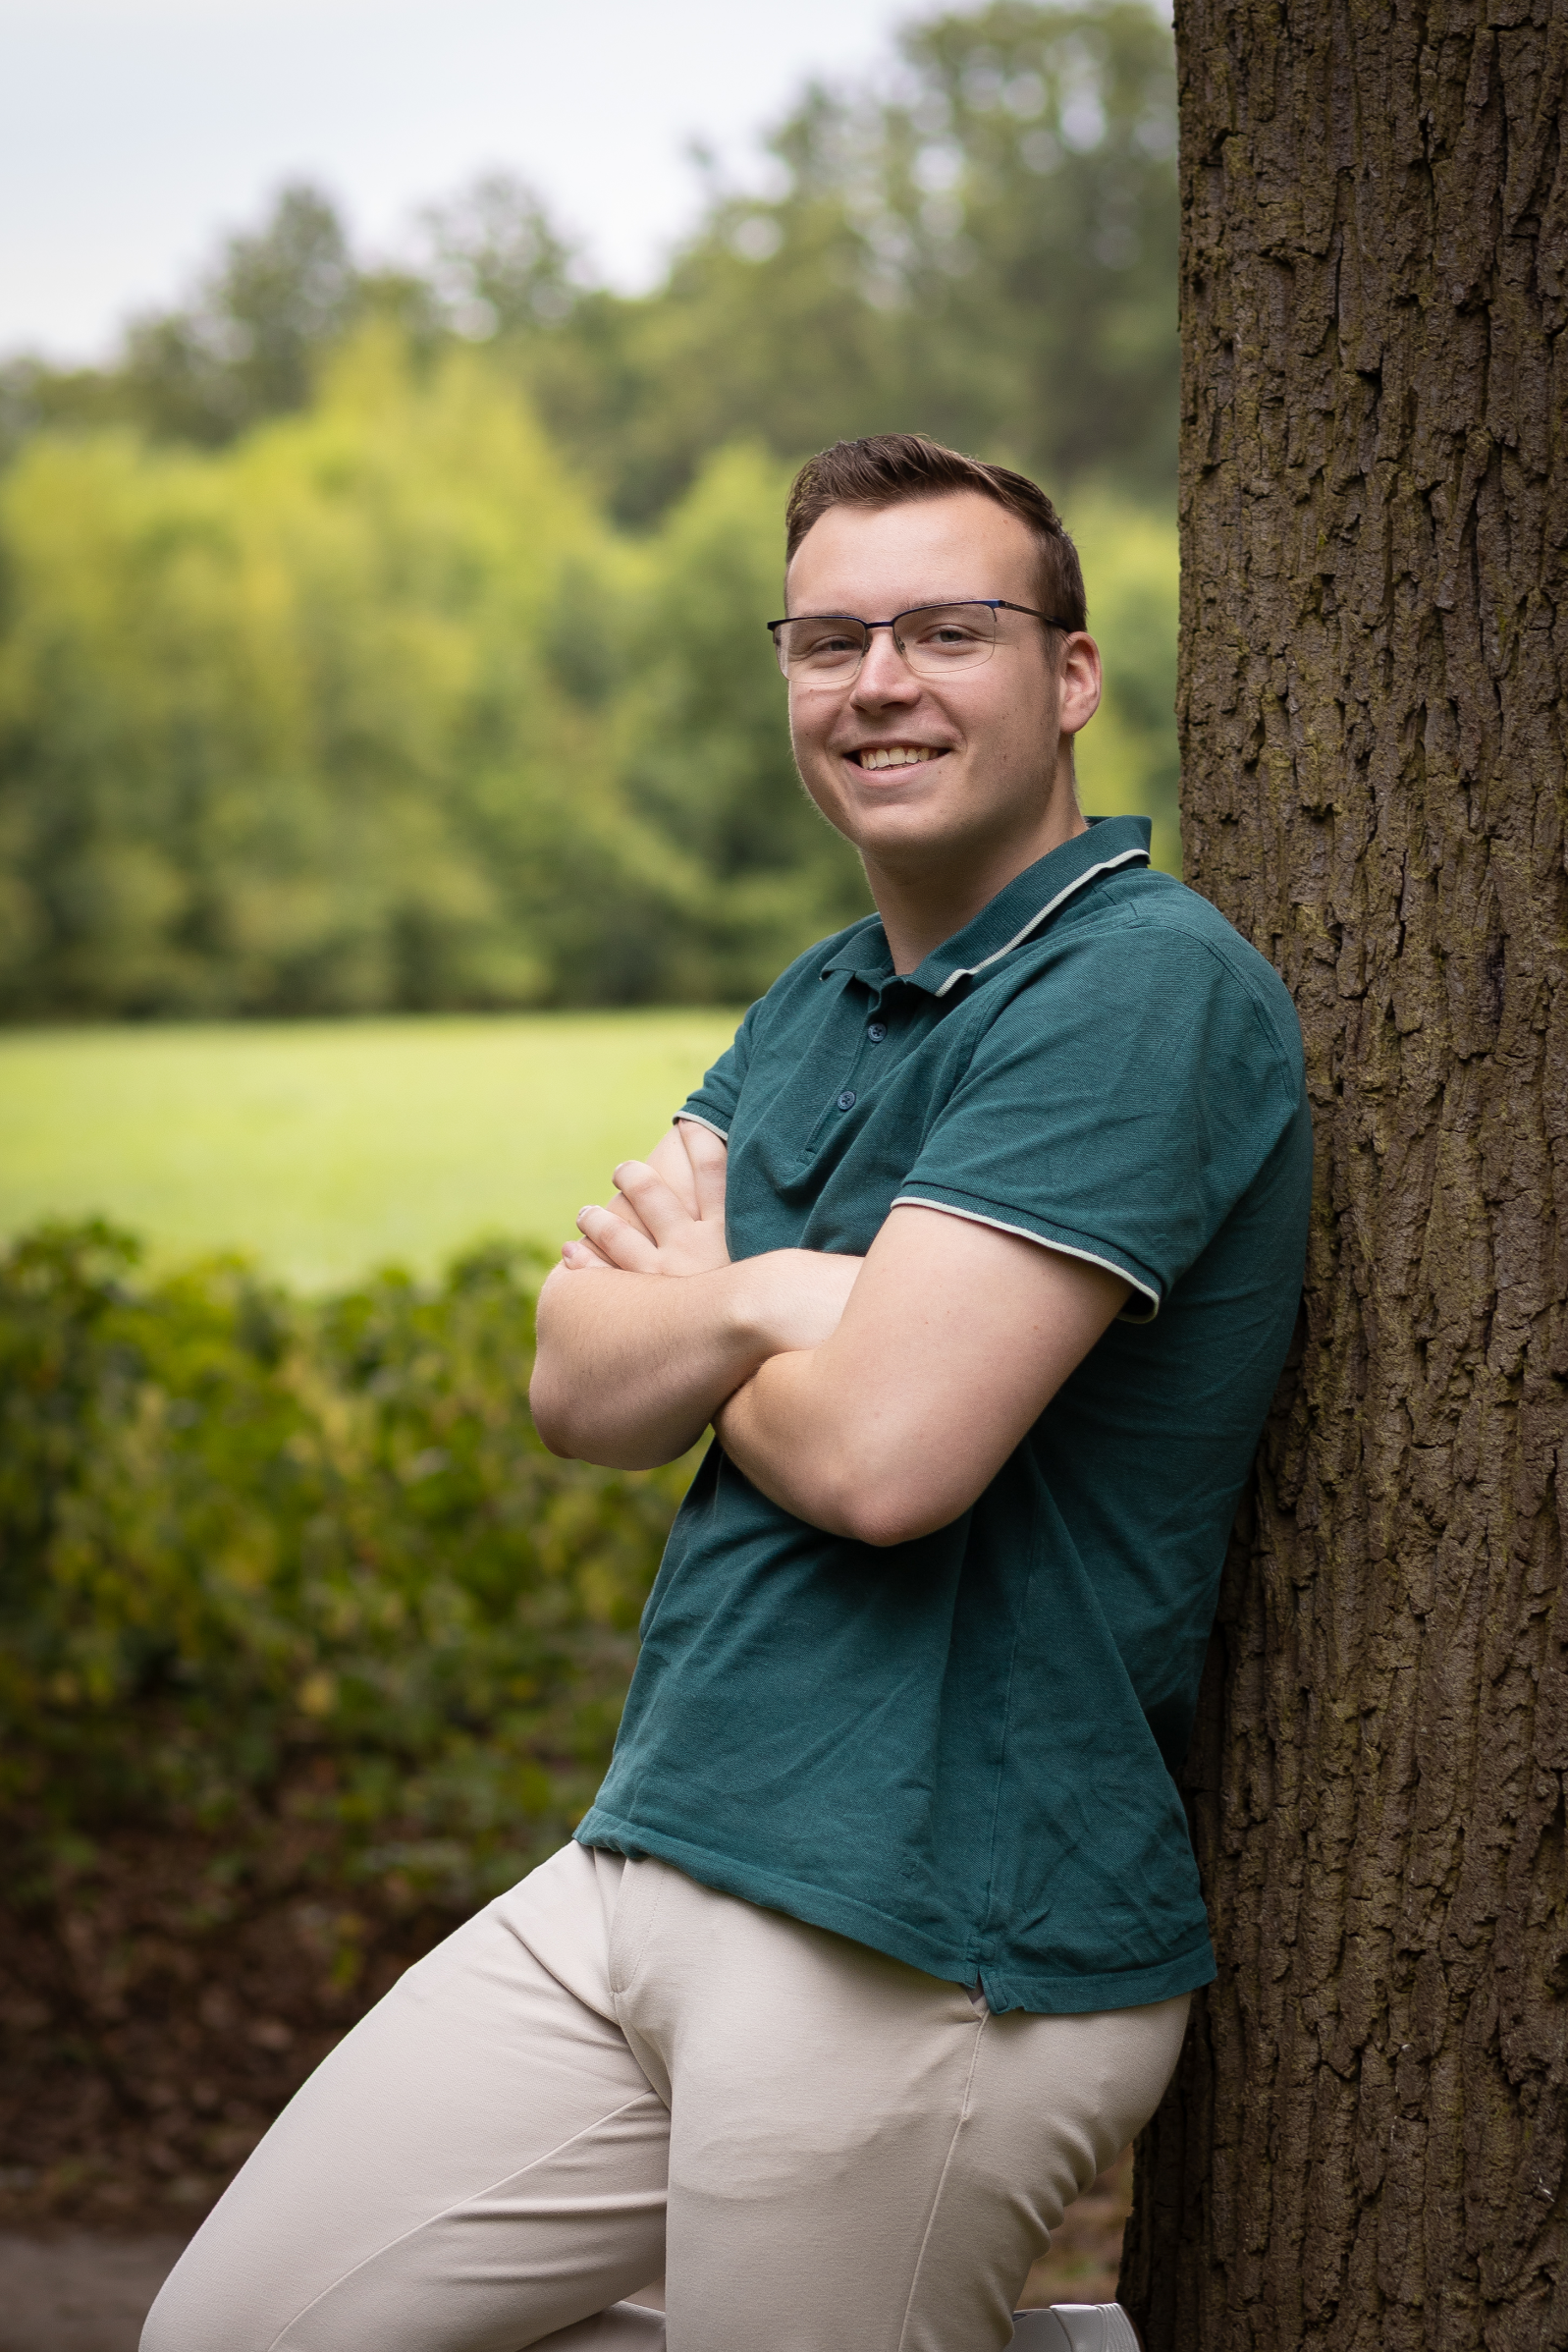
\includegraphics[width=2.6cm]{./assets/picture.png}};
  \end{tikzpicture}
\end{minipage}

\vspace{4pt}

% ═══════════════════════════════════════════════════════════
% PROFIEL
% ═══════════════════════════════════════════════════════════
\section{Profiel}

Backend-gerichte softwareontwikkelaar met 3+ jaar productie-infrastructuurervaring en een sterke interesse in gedistribueerde systemen, event-driven architecturen en backend API-ontwerp.
Thuis in de volledige deployment stack --- van Cisco/VLAN-netwerken en Linux-serverbeheer tot ASP.NET Core API's en message-driven backends.
Studeert momenteel Informatica (HBO) aan Avans Hogeschool en werkt parttime als System Support Engineer bij Dentech.

% ═══════════════════════════════════════════════════════════
% WERKERVARING
% ═══════════════════════════════════════════════════════════
\section{Werkervaring}

\cventry{Dentech Telecommunicatie, Beveiliging \& Automatisering}{Etten-Leur, NL}%
        {System Support Engineer · Parttime}{mei 2024 -- heden}
\begin{itemize}
  \item Beheer van multi-site netwerkinfrastructuur voor 10+ zakelijke klanten via Cisco-switching, VLAN-segmentatie, inter-VLAN routing en firewallbeleid
  \item Beheer van Linux- en Windows Server-omgevingen (Active Directory, Group Policy, DNS/DHCP) en verkorting van provisioning-doorlooptijd met PowerShell- en Bash-automatisering
  \item Implementatie en beheer van Proxmox-virtualisatieclusters met productie-workloads voor klantomgevingen
  \item Leiding over uitrol en configuratie van 3CX PBX-systemen en VoIP-infrastructuur bij nieuwe klantimplementaties
\end{itemize}

\vspace{4pt}

\cventry{Dentech Telecommunicatie, Beveiliging \& Automatisering}{Etten-Leur, NL}%
        {Junior Support Engineer · BBL}{nov 2022 -- mei 2024}
\begin{itemize}
  \item Oplossen van hardware-, software- en VoIP-incidenten in meerdere klantomgevingen, naast het afronden van MBO Niveau 4 ICT Systeem- \& Devicetechnicus
  \item Ondersteuning van Windows Server en Active Directory; opbouw van kerninfrastructuurvaardigheden onder begeleiding van senior collega's
\end{itemize}

% ═══════════════════════════════════════════════════════════
% PROJECTEN
% ═══════════════════════════════════════════════════════════
\section{Projecten}

\cvsimple{PatientPingeling \textnormal{\small\color{taggray}--- \href{https://github.com/PatientPingeling/PatientPingeling}{github.com/PatientPingeling/PatientPingeling}}}{2024 -- heden}
\begin{itemize}
  \item Gebouwd een multi-tenant notificatieplatform met ASP.NET Core, PostgreSQL en RabbitMQ voor berichtrouting via e-mail, SMS en push
  \item Ontworpen provider-abstractielaag voor pluggable notificatieproviders met per-tenant configuratie, zodat nieuwe kanalen geen aanpassingen in de kerndispatch vereisen
  \item Notificatieverzending ontkoppeld van de request lifecycle via RabbitMQ-backgroundconsumers, wat de betrouwbaarheid onder belasting verbetert
  \item Gedistribueerde tracing, metrics en gestructureerde logging toegevoegd via OpenTelemetry; gedeployed via Docker Compose
\end{itemize}

\vspace{4pt}

\cvsimple{Persoonlijke Portfolio --- \href{https://danielvanginneken.nl}{danielvanginneken.nl}}{2025}
\begin{itemize}
  \item Persoonlijke website gebouwd met React en TypeScript; self-hosted via Docker op eigen infrastructuur
\end{itemize}

% ═══════════════════════════════════════════════════════════
% TECHNISCHE VAARDIGHEDEN
% ═══════════════════════════════════════════════════════════
\section{Technische Vaardigheden}

\begin{tabularx}{\textwidth}{@{}>{\bfseries\small}l@{\hspace{10pt}}X@{}}
Backend         & C\# / .NET, ASP.NET Core, Entity Framework Core, REST API's, PostgreSQL, SQL Server \\[3pt]
Messaging       & RabbitMQ, asynchrone verwerking, event-driven architecturen \\[3pt]
Frontend        & React, TypeScript, JavaScript \\[3pt]
Observability   & OpenTelemetry, metrics, tracing, gestructureerde logging \\[3pt]
Infrastructuur  & Linux, Proxmox, VMware, Hyper-V, Docker, Windows Server, Active Directory, PowerShell, Bash \\[3pt]
Netwerken       & Cisco IOS, VLAN's, inter-VLAN routing, firewalls, VPN, DNS/DHCP, 3CX PBX \\[3pt]
Tools           & Git, CI/CD, Azure, Agile / Scrum \\
\end{tabularx}

% ═══════════════════════════════════════════════════════════
% CERTIFICERINGEN
% ═══════════════════════════════════════════════════════════
\section{Certificeringen}

\begin{itemize}[leftmargin=12pt]
  \item Microsoft 365 Certified: Fundamentals (MS-900)
  \item 3CX Advanced Certified Engineer
  \item Yealink Junior Certified IP Phone Engineer
\end{itemize}

% ═══════════════════════════════════════════════════════════
% OPLEIDING
% ═══════════════════════════════════════════════════════════
\section{Opleiding}

\cventry{Bachelor of Applied Science -- Informatica (HBO)}{sep 2024 -- jun 2028}%
        {Avans Hogeschool, Breda}{}

\vspace{4pt}

\cventry{MBO Niveau 4 BBL -- ICT Systeem- \& Devicetechnicus}{sep 2022 -- jun 2024}%
        {Curio, Breda}{}
\vspace{-1pt}
{\small\color{lightgray}Versneld duaal traject: fulltime werkzaam bij Dentech gecombineerd met formele ICT-systeemopleiding}

% ═══════════════════════════════════════════════════════════
% TALEN
% ═══════════════════════════════════════════════════════════
\section{Talen}

Nederlands --- Moedertaal \quad Engels --- Professioneel werkend

\end{document}
